\documentclass[review]{elsarticle}
\usepackage[utf8]{inputenc}
\usepackage{graphicx}
\usepackage{amsmath}
\usepackage{caption}
\usepackage{float}
\usepackage{geometry}
\usepackage{booktabs}
\usepackage{siunitx}
\usepackage{pgfplots}
%\usepackage{authblk} % To include affiliations of authors
\usepackage{url}
\usepackage{chemformula} % Formula subscripts using \ch{}
%\usepgfplotslibrary{groupplots}
\pgfplotsset{compat=1.18} % 
\usepackage{xcolor}
\usepackage{comment}
\usepackage{diagbox}
\usepackage{ulem}

\newcommand{\gc}{\mathrm{g_c}}
\newcommand{\vc}{\mathrm{v_c}}
\newcommand{\ugc}{$\mathrm{ug_c}$}
\newcommand{\uvc}{\mathrm{uv_c}}



\begin{document}
\captionsetup[figure]{labelfont={bf},labelformat={default},labelsep=period,name={Fig.}}

\begin{frontmatter}

\title{\sout{Prediction of the Structural Properties of MOFs with High Hydrogen Storage Capacities at Room Temperature and Moderate Pressures using Neural Networks} \textcolor{red}{Inverse Design of Metal–Organic Frameworks for Hydrogen Storage at Room Temperature and Moderate Pressure Using Neural Networks}}
\date{}
\author[1]{A. Granja-DelRío \corref{corr}}
\cortext[corr]{Corresponding author}
\ead{alejandra.granja@uva.es}
\author[1]{I. Cabria}
\author[2]{T. Calonge}
\address[1]{Departamento de F\'{\i}sica Te\'orica, At\'omica
y \'Optica, Universidad de Valladolid, ES-47011 Valladolid, Spain}
\address[2]{Departamento de Informática (ATC, CCIA y LSI),
Universidad de Valladolid, ES-47011 Valladolid, Spain}



\begin{abstract}
Metal-Organic Frameworks (MOFs) are promising 
solid porous materials for hydrogen storage at 
room temperature and low or moderate pressures for Fuel Cell Vehicles (FCVs). Study and exploration of the hydrogen storage capacities of MOFs and other solid porous materials using Grand Canonical Monte Carlo (GCMC), Density Functional Theory (DFT) and other methods are computationally expensive. An Artificial Neural Network (ANN) approach is presented and trained on a dataset of 1000 MOFs, obtained from GCMC simulations of the MOFs at 298.15 K and 25 MPa. More precisely, each sample contains the hydrogen usable gravimetric and volumetric capacities at that temperature and pressure and five structural properties of the 1000 MOFs. The aim of the ANN is to find the Structural Properties of one or more MOFs whose hydrogen usable volumetric and gravimetric storage capacities at 298.15 K and 25 MPa are consistent with the Department of Energy (DOE) hydrogen storage targets for 2025. \sout{In practice, the problem formulation is just the opposite: Use Machine Learning (ML) methods to find/obtain the hydrogen usable storage capacities of MOFs, using a dataset of known MOFs. The ANN is used to find an input space region (structural properties region) where a solution (a MOF with given hydrogen usable gravimetric and volumetric capacities at 298.15 K and 25 MPa equal to the DOE targets) could be searched for. GCMC simulations of some MOFs close to the found input space region of structural properties have been also performed. The usable gravimetric capacities are close to the given capacities, but not to the usable volumetric capacities. }
\textcolor{red}{
Unlike conventional Machine Learning (ML) algorithms that directly predict hydrogen uptake from structural descriptors, the present work formulates the problem in an inverse design manner, using an ANN to identify regions of the structural-property space compatible with target storage performances. This strategy enables the rapid screening of candidate MOFs and provides physically interpretable guidance for materials discovery.}

\end{abstract}


\end{frontmatter}

%%%%%%%%%%%%%%%%%%%%%%%%%%%%%%%%%%%%%%%%%%%%%%
\section{Introduction}
%%%%%%%%%%%%%%%%%%%%%%%%%%%%%%%%%%%%%%%%%%%%%%

Transport is essential for modern life. It connects people and supports trade, culture, and access to basic services. However, it also has strong negative impacts. It is responsible for about 25 \% of greenhouse gas emissions in the EU \cite{zjb+24,cde+22,jena11}, and it increases air and noise pollution as well as habitat loss \cite{tm24}. For this reason, cleaner energy solutions are needed.

Hydrogen is seen as a good alternative for reducing emissions. In vehicles, it can replace fossil fuels, especially in Fuel Cell Vehicles (FCVs). Its gravimetric energy density is very high, 120 MJ/kg, while gasoline offers only 44 MJ/kg \cite{doe25}. However, the volumetric energy density is low at ambient conditions and moderate pressures (0.5–25 or 35 MPa). This makes onboard storage a difficult challenge. Current systems compress hydrogen up to 70 MPa \cite{atd20}, 
\sout{which increases costs and safety concerns.}
\textcolor{red}{which is common in commercial compressed-gas storage technologies, but increases cost, system complexity, and safety requirements.}

To face this problem, the US Department of Energy (DOE) defined targets for 2025. They require at least 5.5 wt. \% for the usable gravimetric capacity, $\ugc$, and 0.040 kg/L for the usable volumetric capacity, $\uvc$ \cite{doe25,ahg+18}. These values are considered essential for real applications, where driving ranges above 600 km are needed \cite{cwlcz23,bww+21,breeze18,hv14,dy11}.

Among possible storage materials, Metal-Organic Frameworks (MOFs) are very promising. They combine high surface area, tunable pore sizes, and flexible design. This makes them good candidates for hydrogen storage near room temperature through physisorption \cite{gc24}. Still, finding new MOFs that meet both gravimetric and volumetric targets is not straightforward. It often requires extensive experimental work or computationally demanding simulations such as Grand Canonical Monte Carlo (GCMC) and Density Functional Theory (DFT) \cite{ltc24,cltgv21}.

\textcolor{red}{
In recent years, \sout{machine-learning} ML techniques have been extensively applied to accelerate the prediction of hydrogen storage properties in MOFs and other porous materials. Previous studies have explored the use of \sout{artificial neural networks} ANN like random forests, and other regression models to predict hydrogen uptake or deliverable capacities from structural descriptors \cite{gm21,sra23,qxx+24,cbc+25,as21,wwyq25,sra23}. These approaches have demonstrated that data-driven models can significantly reduce the computational cost associated with high-throughput GCMC or DFT simulations.}
\textcolor{blue}{Qué previous?}

\textcolor{red}{
However, most existing studies focus on the direct prediction of hydrogen storage performance from known structural features, effectively addressing a forward-design problem. In contrast, less attention has been paid to the inverse formulation, where desired storage targets are used to infer regions of the structural-property space that could host suitable materials. This limitation restricts the direct applicability of \sout{machine-learning} ML models as design-guidance tools for experimental synthesis.}


Tens of thousands of synthesized MOFs and millions of theoretical and 
not synthesized MOFs have been reported \cite{llk+22, spst21}. Their large 
diversity and the use of different metals give researchers many options to design new structures with high potential for hydrogen storage.

\sout{From a mathematical point of view, a search in a solutions space must be taken place, in order to find materials to construct an adequate Hydrogen Cell Vehicle.}
\textcolor{red}{From a computational perspective, the identification of suitable MOFs for onboard hydrogen storage can be formulated as a search problem within a high-dimensional materials space.}
To do that, a MOFs table will be available. Each row will store the characteristic parameters of a given material. The mentioned GCMC will provide the corresponding $\uvc$ and $\ugc$, as it will be described in the following section. All this information will make up the dataset for any \sout{Machine Learning} ML algorithm, in this work, used as regression system, also know as function estimator \cite{geron2019}. \textcolor{red}{In particular, an approach based on ANN will be presented, but previously other ML function estimators  have been tested and discarded such as decision tree or support vector machine based prototypes.}  

The ANN will be trained using a dataset composed by the usable storage capacities at 298.15 K and 25 MPa plus five structural properties of 1000 MOFs. The usable capacities were obtained by means of GCMC simulations performed using an in-house code published in GitHub \cite{mcmgs}.
When ANNs are applied in the field of materials science, the usual procedure is as follows: the structural parameters of the materials are the inputs and the desired capabilities of the materials are the outputs. \sout{In this work, the problem statement will be the opposite:}
\textcolor{red}{In this work, an alternative strategy is explored,}
for given $\ugc$ and $\uvc$ (given/desired properties), \sout{the ANN will obtain the five structural parameters of an hypothetical MOF}
\textcolor{red}{the ANN estimates the ranges of five structural parameters of a hypothetical MOF} whose usable storage capacities will be equal or larger than the DOE capacity targets for 2025. Finally, GCMC simulations of MOFs whose structural properties are close to the structural properties predicted by the ANN, will be also performed and analyzed.

\textcolor{red}{The main novelty of the present work lies in formulating hydrogen storage optimization in MOFs as an inverse-design problem at near-ambient temperature and moderate pressure. Instead of predicting storage capacities from given structures, the ANN is used to identify regions of the structural-parameter space that are consistent with DOE performance targets. This shift from forward prediction to inverse mapping provides actionable guidance for materials design and complements existing high-throughput screening methodologies.
}


\textcolor{red}{
This work builds upon previous data-driven studies while explicitly positioning the ANN as a complementary tool to conventional high-throughput screening approaches rather than as a replacement for detailed molecular simulations.}


%%%%%%%%%%%%%%%%%%%%%%%%%%%%%%%%%%%%%%%%%%%%%%
\section{Methodology}
%%%%%%%%%%%%%%%%%%%%%%%%%%%%%%%%%%%%%%%%%%%%%%

%%%%%%%%%%%%%%%%%%%%%%%
\subsection{Grand Canonical Monte Carlo Simulations}
%%%%%%%%%%%%%%%%%%%%%%%

Grand Canonical Monte Carlo (GCMC) simulations were performed to evaluate the total and 
usable hydrogen gravimetric and volumetric storage capacities of MOFs chosen from the Cambridge Crystallographic Database Centre (CCDC) \cite{ccdc}. The simulations were carried out at 298.15 K with pressures at 0.5 and 25 MPa.

Each GCMC run consisted of ten millions steps. The first five millions were used to reach equilibrium, and the last five millions were employed to calculate the storage values. The Metropolis algorithm was applied during all iterations \cite{metropolis87}. The types of moves on each iteration were assigned with the following probabilities, after running some tests: 20 \% for molecular displacement, 40 \% for deletion, and 40 \% for insertion \cite{cc22,gc24,gc24a}.

The chemical potential was determined with the Soave–Redlich–Kwong (SRK) equation of state \cite{soave72}. The values for the acentric factor $\omega$, the critical pressure $P_c$, and the critical temperature $T_c$ of hydrogen and methane were taken from Zhou and Zhou \cite{zz01} and Xu et al. \cite{xdy12}.

The interactions between the framework atoms and the gas molecules were described with Lennard–Jones (LJ) potentials \cite{lennard24}. The LJ parameters were calculated using the Good-Hope combining rule for $\sigma$ \cite{gh70} and the Berthelot rule for $\epsilon$ \cite{berthelot1898}. \textcolor{red}{Specific LJ parameters were used for the C and \ch{H2} interaction, without applying the Berthelot-Good Hope combining rule.} The values of the LJ parameters of the atoms and molecules used in 
the simulations can be found in GitHub \cite{mcmgs}. \textcolor{red}{The cutoff radius was set to 20 \AA{}, after running several tests \cite{cc22,gc24,gc24a}. In the GCMC simulations, the atoms that composed the MOFs were treated as rigid.}

All simulations were executed using an in-house program, published in GitHub and written in fortran \cite{mcmgs}. \textcolor{red}{
The in-house GCMC code employed in this work has been previously validated against both
experimental measurements and results obtained with established simulation packages,
including RASPA, for hydrogen adsorption in benchmark MOFs.
In particular, systematic comparisons for materials such as IRMOF-1, IRMOF-20, and ZIF-8
under a wide range of temperatures and pressures have been reported in previous studies,
showing good agreement in both gravimetric and volumetric storage capacities
\cite{gc24a,gc24b,gc24c,gc25a}.}

\textcolor{red}{
These validation studies demonstrate that the present implementation reliably reproduces
the magnitude and trends of hydrogen adsorption reported in the literature.
The use of in-house GCMC codes for large-scale screening has also been adopted in earlier
works, as it provides greater flexibility and reduced computational cost when exploring
high-dimensional materials spaces.
While widely used software packages such as RASPA \cite{dces16} remain a reference tool for
adsorption simulations, the present implementation offers comparable accuracy for the
purposes of comparative screening and inverse property mapping considered in this work.
}

The input of the program for each MOF consisted mainly on the cell of the MOF, obtained from the CIF (Crystallographic Information File) file on the CCDC database. Part of the input was also the number of iterations, the probabilities of the types of moves, the type of equation state (SRK in the present case) and the cutoff radius. The program calculates the total and usable volumetric and gravimetric storage capacities, which are defined in the next paragraphs.

\textcolor{red}{Prior to the GCMC simulations, all MOF structures obtained from the CCDC were carefully prepared for computational use. Solvent molecules and non-framework species were removed from the CIF files, and the structural integrity of the frameworks was verified by checking atomic positions and unit cell parameters. As a result, all structures used in this work are computation-ready and equivalent in quality to those provided by curated databases such as the CoRE MOF database.
}

The five structural parameters of each MOF were obtained by means of the 
Zeo++ code \cite{zeoplusplus}. Those parameters were: the density in kg/L, 
the porosity (a dimensionless magnitude; its values are between 0 and 1), 
the radius of the largest pore of the MOF, $R_i$, in \AA{}, the specific 
surface area, SSA, in m$^2$/g, and the specific pore volume, SPV, in cm$^3$/g.

%%%%%%%%%%%%%%%%%%%%%%%
\subsubsection{Definitions of Storage Capacities}
%%%%%%%%%%%%%%%%%%%%%%%

In these simulations, the total volumetric storage capacity of hydrogen gas at pressure $P$ and temperature $T$, $\vc(P,T)$, also referred to as the density of stored gas, is expressed as

\begin{equation}
\label{vc}
\vc(P,T) = \frac{M_g(P,T)}{V} \;,
\end{equation}

\noindent
where $M_g(P,T)$ corresponds to the total mass of gas (hydrogen) stored inside the simulation box at pressure $P$ and temperature $T$, and $V$ denotes the box volume. In this work, $\vc$ is reported in units of kg of \ch{H2}/L.

The total gravimetric storage capacity at pressure $P$ and temperature $T$, $\gc$$(P,T)$, is determined from

\begin{equation}
\label{gc}
\gc(P,T) = \frac{100 M_g(P,T)}{M_g(P,T) + M_{ads}} \;,
\end{equation}

\noindent
with $M_{ads}$ represents the mass of the porous adsorbent material contained in the simulation cell, respectively. The total $\gc$ is expressed in weight percent (wt. \%).

The usable gas mass at $P$ and $T$, $M_{ug}(P,T)$, is defined as the difference between the total gas mass stored at a given pressure $P$ and temperature $T$ and the gas mass that remains at the lower (depletion) pressure, $P_{dep}$, at the same $T$, 
$M_{ug}(P,T)$ = $M_g(P,T) - M_g(P_{dep},T)$. 
\textcolor{red}{In this work, the depletion pressure was set to $P_{dep} = 0.5$ MPa, consistent with values used in the literature for defining usable or working hydrogen storage capacities in adsorption systems. This choice corresponds to the lower bound of pressures accessible in typical fuel cell operation \cite{cltgv21,rscf22}.}
The usable volumetric and gravimetric capacities, also called working or deliverable capacities \cite{doe25,ahg+18,sh16}, follow directly from Eqs.~\ref{vc} and~\ref{gc}, respectively, replacing the total mass, $M_g(P,T)$, by the usable mass, $M_{ug}(P,T)$, into the definitions. The usable and 
total capacities have the same corresponding units: gravimetric in wt. \% and volumetric in kg/L. In this study, only the usable storage capacities are considered and discussed.

%%%%%%%%%%%%%%%%%%%%%%%
\subsection{Dataset}
%%%%%%%%%%%%%%%%%%%%%%%

\sout{The ANN} \textcolor{blue}{Several ML systems were considered and implemented using a dataset of 1000 MOFs}, which was structured as a table with seven columns and 1000 rows, was generated from GCMC simulations at 0.5 MPa and 25 MPa performed on MOFs randomly selected from the CCDC database. Each row represents one MOF and contains: the two usable capacities ($\ugc$ in wt.\% and $\uvc$ in kg/L at 298.15 K and 25 MPa) and the five basic structural parameters. In this work, the ANN takes the two usable capacities as inputs and predicts the five structural magnitudes as outputs.

%%%%%%%%%%%%%%%%%%%%%%%
\subsection{Machine Learning Regression}\label{Machine Learning Regression}
%%%%%%%%%%%%%%%%%%%%%%%
\textcolor{blue}{Considero que en metodología solo se definen los métodos, no se hacen pruebas para seleccionarlo, esta parte va en resultados, para decir por qué se coge uno u otro}

\textcolor{red}{ML Theory originally formulated two fundamental supervised learning challenges: classification and regression \cite{hastie2009elements, bishop2006}.  From an external data point of view, the difference between them lies simply in the numerical type of the desired output associated with each input. In effect, for classification problems, the output needs to be discrete while for regression, it must be continuous \cite{mitchell97}.}  From decision trees up to some of approaches belonging to the large group called "Linear Methods" have both classification and regression version. Without a doubt, the most relevant examples for that application are in the ANN category, since they could simulated a wide variety of functions  even if a high no linearity will be present \cite{witten2011data}.

\textcolor{blue}{Before model training, an experimental protocol and evaluation metric were defined. A Hold-Out strategy with a 2/3–1/3 split between training and testing sets was adopted as an initial validation procedure \cite{hastie2009elements}. The coefficient of determination, R$^2$, was selected as the primary regression metric, as it provides a direct measure of the proportion of variance explained by the model \cite{james2021}.}


\textcolor{blue}{\textcolor{red}{In order to define an appropriate regression framework for the present problem, several widely used supervised learning regressors were considered, following standard practice in the literature \cite{witten2011data}:
\begin{itemize}
    \item Decision Tree Regressor (DTR)
    \item Support Vector Machine with a gaussian kernel (SVR)
    \item Multilayer Perceptron (MLP-R)
\end{itemize}

The first two prototypes were programmed in Python using the scikit-learn module. Due to their implementation requirements, it was necessary to handle a list of individual regressor: one for each output. Each list of these ML regressor was integrated into a single object, for which the typical methods (\_\_init\_\_, fit, predict, and score) were implemented.

Respect to the last algorithm (MLP-R), it was opted for direct PyTorch implementation rather than using the corresponding scikit-learn module. This decision was driven by PyTorch's superior flexibility, which allowed us to experiment with different activation functions across distinct layers \cite{raschka2020machine}.  

%%%%%%%%%%%%%%%%%%%%%%%
\subsection{Multilayer Perceptron Regressor}
%%%%%%%%%%%%%%%%%%%%%%%

Following the Multilayer Perceptron, (MLP) architecture, an artificial neural network is proposed as final prototype. As it can be seen in Fig. \ref{regressor}, the model has the same size (ten neurons) for the hidden layers. The number of nodes for the rest of layers are adjusted according to the input and output vectors dimensions. Respect to the activation functions for each layer, it is necessary to take in mind that it is a regression problem, which implies to use the identity as activation function in the output. For the hidden layers, an activation function is needed to be chosen. That function must be restricted to be continuous, bounded and monotonically  increasing, in order to maintain the numerical stability of the system \cite{haykin1999neural}. In addition, because the training algorithm is based on the gradient operation, this activation function has to be differentiable. Finally, the parameters calculated by the model correspond to physical magnitudes that doesn't admit negative or null values. For all these reasons, the choice of the activation function will be the sigmoid, also known as logistic function \cite{bishop1995mlp}.

\begin{figure}[ht]
    \centering
    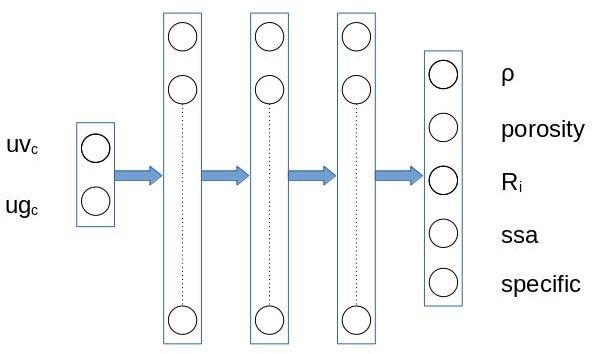
\includegraphics[width=0.75\linewidth]{Arquitectura MLP Recortado.jpg}
    \caption{MLP Regressor Architecture}
    \label{regressor}
\end{figure}


\textcolor{blue}{After the hyperparameter exploration stage, the selected MLP architecture is retrained using the full dataset. In this final training step, all available samples are combined to build a single regression model, ensuring that the maximum amount of information is used. This procedure is standard practice once model configuration has been fixed, and it avoids unnecessary loss of training data due to validation splits.}

The rest of implementation details  correspond to computation topics. First of all is the programming language and the interactive development environment (IDE). In this particular case, both Python and Jupyter were chosen. However, the most relevant tool for the ANN was PyTorch \cite{pytorch}, which has been built upon tensor calculus to enable an efficient and flexible Deep Learning computation. All the proposed model programs were prepared to be executed automatically on both CPU and GPU; the last option only works if a corresponding hardware device is available and compatible with the CUDA\footnote{Compute Unified Device Architecture - NVIDIA's parallel computing platform and programming model.}or ROCm\footnote{ROCm: AMD's open-source alternative to NVIDIA's CUDA.} version used by PyTorch.

Under that configuration, the system must tune the total amount of 305 trainable parameters. Due to a 900 training samples corresponding to corresponding to 9 of 10 Cross-Validation folds  (see next paragraph),each of them with five attributes, it will avoid the under-training risk, since the inputs per weight (6) is more than enough \cite{vapnik1999nature}.

Regarding the experimental methodology, Cross-Validation was chosen instead of the Hold-Out method used in the preceding subsection. Hold-Out was adequate there because only a single numerical value was required for preliminary comparison and model screening. However, to draw reliable conclusions, a single Hold-Out split is insufficient; multiple experiments with varying train/test splits are necessary. Repeated Hold-Out could be a viable solution, as the variance of the estimate does not depend on a single split but is distributed across multiple experiments. Cross-Validation offers a similar advantage but with a key benefit: it ensures that all samples are used for both training and testing. This property cannot be guaranteed by Repeated Hold-Out \cite{james2021}.

Previously, each input and output was scaled into the interval [0,1]. In this step, there is only one thing left to do with samples: organizing them into batches. With the aim to avoid any rote learning, the samples will be permuted in each epoch. As it is well known, this task is the foundation for every Stochastic Optimization process, that will also improve the power of generalization, which is the main goal of any machine learning system \cite{bottou2018optimization}.

To execute the algorithm, it is necessary to set some optimization issues. The most important is the cost function. In a regression problem, the Mean Squared Error (MSE) is a very good candidate for assessing optimization and performance \cite{bishop2006}. The next step consists on the optimizer election according to the preceding lost function. The Adaptive Moment Estimation (ADAM) is probably the most popular ANN optimizer \cite{choi2020survey}. It is based on gradients that include not just the momentum term in an adaptive manner, but also incorporates several regularization algorithms like L1 and L2 \cite{kingma2015adam}.

The model implementation was split into two phases:
\begin{itemize}
    \item Hyperparameters setting
    \item Production mode
\end{itemize}

\textcolor{red}{The first methodology requires extensive trial-and-error experimentation, guided by empirical rules, to identify suitable MLP hidden layer architectures and optimizer hyperparameters (e.g., learning rate, momentum, and regularization coefficients). This represents the most computationally expensive phase, as the number of trials is multiplied by the number of cross-validation folds (10).}  



%%%%%%%%%%%%%%%%%%%%%%%%%%%%%%%%%%%%%%%%%%%%%%%%%%%%%%%%%%
\section{Results and Discussion}
%%%%%%%%%%%%%%%%%%%%%%%%%%%%%%%%%%%%%%%%%%%%%%%%%%%%%%%%%%

The table \ref{tab:placeholder} presents the comparison results for each prototype. Only the coefficient of determination (R$^2$) values obtained for the test dataset are shown, as this is the most important metric in the ML environment, given its direct relationship to the generalization power of systems \cite{goodfellow2016deep}.

\begin{table}[H]
    \centering
    \begin{tabular}{|c|c|c|c|}\hline
         ML regressor:&  DTR&  SVR& MLP-R\\\hline
         R²&  0.8234&  0.5495& 0.8723\\ \hline
    \end{tabular}
    \caption{R² comparison for several ML regressors}
    \label{tab:placeholder}
\end{table}

\textcolor{red}{Consequently, based on Table \ref{tab:placeholder}, the prototype chosen for the final implementation is MLP-R. As with the previous two systems, a corresponding object with the typical PyTorch  "\_\_init\_\_ " and "forward" methods has also been created (detailed in the next section). At a more abstract level, the five outputs are not independent; instead, they are integrated into a single MLP. This enables the modeling of potential cross‑dependencies among output variables, which the two previous systems ignore.}

\textcolor{red}{To further assess the robustness and stability of the selected MLP regressor, a 10-fold cross-validation procedure was performed.}

\textcolor{red}{Table \ref{tab:CV MLP-R} summarizes the results from the best-tested hyperparameter set.}}
\begin{table}
    \centering
    \begin{tabular}{lrccc}\toprule
 FOLD (CV)& MSE (train)& MSE (test)& R² (train)&R²(test)\\\midrule
          0&0.002066&  0.002056&  0.885354&  0.898407\\
          1&0.002214&  0.002417&  0.858594&  0.844268\\
          2&0.002134&  0.003154&  0.883937&  0.878659\\
          3&0.002033&  0.001567&  0.898638&  0.875035\\
          4&0.002206&  0.001871&  0.856156&  0.837287\\
          5&0.001999&  0.001691&  0.910156&  0.909507\\
          6&0.002044&  0.002102&  0.893892&  0.893620\\
          7&0.001790&  0.003677&  0.886273&  0.858905\\
          8&0.001878&  0.002324&  0.870179&  0.879475\\
          9&0.002053&  0.001649&  0.859180&  0.854832\\
 \textbf{Average}& \textbf{0.002042}& \textbf{0.002251}& \textbf{0.880236}&\textbf{0.872999}\\ \bottomrule
    \end{tabular}
    \caption{Cross Validation MLP-Regressor Results}
    \label{tab:CV MLP-R}
\end{table}

\textcolor{red}{A method to monitor the performance of the ANN regressor is to track the loss function over the training epochs that corresponds to Fig. \ref{mse}. }As it can be seen, both training and test curves are monotonically decreasing over the epochs. They evolve towards asymptotic values below 0.003. Taking into account that every magnitude manged by the model are scaled in the interval [0,1], the mean squared error over the samples is under 0.3 \%. This value can be accepted as reasonable \cite{goodfellow2016deep}.

\begin{figure}[H]
    \centering
    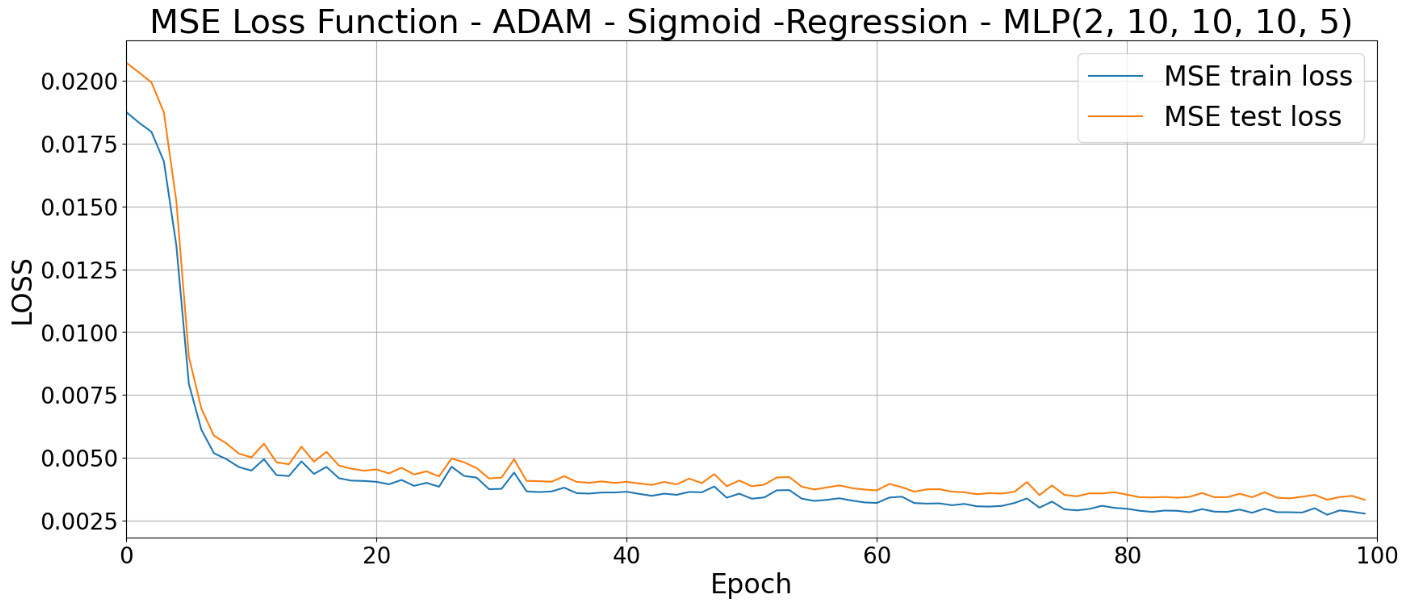
\includegraphics[width=1\linewidth]{MSE Evolution.jpg}
    \caption{MSE evolution of MLP-Regressor}
    \label{mse}
\end{figure}

\textcolor{red}{However, as noted in \ref{Machine Learning Regression}, the key metric for this problem is R². As can be seen in \ref{tab:CV MLP-R}, this parameter is close to 0.9, which can be considered adequate. This result allows us to consider the present approach satisfactory from a Machine Learning perspective.}

%%%%%%%%%%%%%%%%%%%%%%%
\subsection{\textcolor{red}{Inverse Mapping and Identification of Candidate MOFs}}
%%%%%%%%%%%%%%%%%%%%%%%

\textcolor{red}{After determining that the MLP Regressor produces the best results, it can be used as an inverse mapping tool. As mentioned before, the main goal of this  system should be to calculate the structural parameters of a MOF (outputs) for given $\ugc$ and $\uvc$ (inputs). The prototype's response likely doesn't correspond to a real MOF that will allow us to build a practical storage tank for a FCV. However, a region around the outputs could bound the range of the structural parameters of the MOF where a solution is sought (see Fig. \ref{ANN_MOFs_Solution}) or a MOF whose usable capacities are close to the goals can be found.}

\textcolor{red}{In this sense, the ANN should be understood as a guiding tool to delimit promising regions of the structural space, rather than as a direct generator of experimentally realizable materials.}


\begin{figure}[ht]
    \centering
    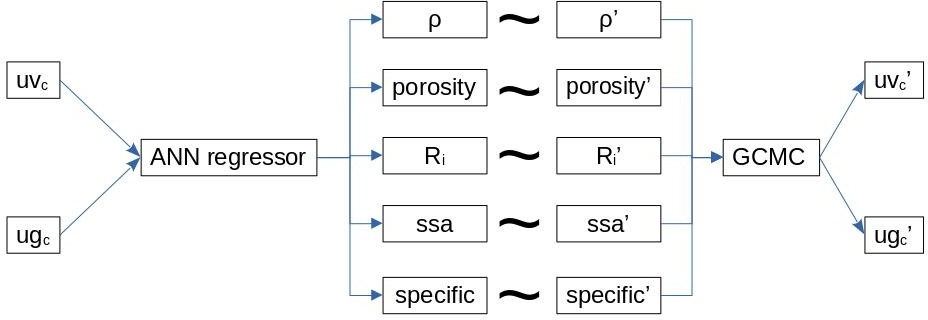
\includegraphics[width=1\linewidth]{Figura Esquema Recortado.jpg}
    \caption{ANN output as starting point to search a MOFs solution}
    \label{ANN_MOFs_Solution}
\end{figure}

\textcolor{red}{Based on the predicted structural parameters, MOFs with similar characteristics were identified within the CCDC database.
Grand Canonical Monte Carlo simulations were then performed for these selected materials at 298.15 K and 25 MPa in order to evaluate their hydrogen storage performance.
The corresponding structural parameters and usable storage capacities are reported in Table~\ref{mofs}.
}

\textcolor{red}{To illustrate the application of the inverse mapping strategy, two representative target pairs of usable gravimetric and volumetric capacities were selected.
}
Table~\ref{outputs} summarize the MOFs structural parameters as output according to the two sets of given (or input) hydrogen $\ugc$ and $\uvc$, obtained using and omitting the Hold-Out methodology.

\begin{table}[H]
    \centering
    \begin{tabular}{ccccccc}
    \hline
\multicolumn{7}{c}{Hold-Out Prototype Outputs}\\
\hline
         $\ugc$   & $\uvc$   & density & porosity & $R_i$ & SSA  & SPV\\
         2.75  & 0.04  & 0.597   & 0.413    & 5.69  & 3562 & 0.567\\
         5.50  & 0.04  & 0.386   & 0.673    & 8.37  & 5166 & 2.125\\
    \hline
\multicolumn{7}{c}{No Hold-Out Prototype Outputs}\\
\hline
         $\ugc$   & $\uvc$   &  density &  porosity &  $R_i$ & SSA  & SPV\\
         2.75  & 0.04  &  1.058   &  0.344    &  4.83  & 2772 & 0.282\\
         5.50  & 0.04  &  0.416   &  0.645    &  8.03  & 4810 & 1.717\\
    \hline
    \end{tabular}
    \caption{Hold-Out and No Hold-Out Prototype Outputs}
    \label{outputs}
\end{table}

The ANN predicted the structural parameters shown in Table~\ref{outputs}. We have inspected the MOFs of the CCDC database and 
have looked for MOFs whose structural parameters match or are close 
to the values predicted by the ANN and presented in that Table. We have found some MOFs in the CCDC database whose structural parameters are close, although not the five parameters are close to the predicted ones. We have performed GCMC simulations of those selected MOFs at 298.15 K and 25 MPa. The CCDC identifiers of those MOFs and their structural parameters and usable storage capacities are shown in Table~\ref{mofs}.

Regarding the computational volume required to train the proposed ANN systems, the elapsed time for 200 epochs of the first system was less than  three minutes on a Linux virtual machine with eight cores of an Intel(R) Xeon(R) Gold 6128 CPU @ 3.40 GHz. It shows that a GPU is not crucial for the present work.

\begin{table}[H]
\begin{center}
\caption{\noindent
\label{mofs} 
Structural parameters and usable storage capacities at 298.15 and 25 MPa of the selected MOFs. The reported parameters include framework density, ($\rho$, kg/L), porosity, (Prs., dimensionless), 
largest pore radius, ($R_i$, \AA), specific surface area (SSA, m$^2$/g), specific pore volume (SPV, cm$^3$/g), usable gravimetric capacity ($\ugc$, wt.\%), and usable volumetric capacity ($\uvc$, kg/L).}
        \begin{tabular}{cccccccc}
\hline
\diagbox{MOF}{Properties} & \textbf{Prs.} & \textbf{$\rho$} & \textbf{$R_i$} & \textbf{SSA} & \textbf{SPV} & \textbf{$\uvc$} & \textbf{$\ugc$}\\
\hline
alejae            &  0.694 &  0.283  &  11.20  & 4795.04 & 2.54398 & 0.0162 & 5.40 \\
bazfuf01          &  0.566 &  0.357  &  11.25  & 5191.53 & 1.67818 & 0.0157 & 4.20 \\
bazfuf            &  0.567 &  0.355  &  11.33  & 5140.92 & 1.74437 & 0.0158 & 4.25 \\
bibxob            &  0.541 &  0.408  &  11.07  & 4641.18 & 1.51819 & 0.0159 & 3.75 \\
bihbax            &  0.688 &  0.334  &   9.96  & 4395.86 & 2.03445 & 0.0173 & 4.92 \\
bognes            &  0.429 &  0.415  &  10.31  & 5648.74 & 1.01184 & 0.0136 & 3.18 \\
dajwet            &  0.621 &  0.295  &  14.88  & 4985.43 & 2.50898 & 0.0154 & 4.98 \\
dimbot            &  0.746 &  0.430  &  14.99  & 1903.14 & 1.72163 & 0.0166 & 3.72 \\
ecokaj            &  0.682 &  0.333  &   8.97  & 3838.23 & 2.03829 & 0.0153 & 4.39 \\
ehijah            &  0.574 &  0.385  &  10.38  & 4589.81 & 1.66174 & 0.0152 & 3.80 \\
fe-pbpta          &  0.669 &  0.411  &  10.09  & 4336.69 & 1.65417 & 0.0179 & 4.17 \\
ipupoa            &  0.551 &  0.403  &  10.58  & 4794.61 & 1.33786 & 0.0154 & 3.67 \\
JLU-MONT1\_JEYTEP &  0.802 &  0.192  &  14.53  & 6034.91 & 4.47919 & 0.0162 & 7.77 \\
JLU-SOF2\_KODPIF  &  0.749 &  0.232  &  14.12  & 4512.98 & 3.28028 & 0.0153 & 6.20 \\
JLU-SOF3\_KODPIF01 &  0.747 &  0.151  &  11.54  & 7243.99 & 5.56697 & 0.0164 & 9.83 \\
lejcio            &  0.612 &  0.326  &  10.35  & 5125.64 & 1.96099 & 0.0156 & 4.56 \\
omusas            &  0.601 &  0.361  &   7.83  & 3822.92 & 1.66278 & 0.0140 & 3.75 \\
opawot            &  0.566 &  0.368  &   7.03  & 4834.32 & 1.35793 & 0.0153 & 4.00 \\
uqoluj01          &  0.613 &  0.357  &  10.14  & 4834.06 & 1.62163 & 0.0156 & 4.19 \\
vetmis            &  0.609 &  0.321  &   5.11  & 5462.80 & 2.30117 & 0.0155 & 4.59 \\
xahput            &  0.755 &  0.186  &  11.83  & 5870.20 & 4.08809 & 0.0162 & 8.01 \\
xahqaa            &  0.779 &  0.176  &  12.31  & 5832.99 & 4.32    & 0.0164 & 8.52 \\
xanlij            &  0.692 &  0.231  &  13.73  & 5706.56 & 3.03037 & 0.0154 & 6.25 \\
\hline
\end{tabular}
\end{center}
\end{table}

%%%%%%%%%%%%%%%%%%%%%%%
\subsection{Illustrative Comparison with a Commercial FCV}
%%%%%%%%%%%%%%%%%%%%%%%

To illustrate the potential system-level implications of the obtained storage capacities, a simplified comparison with a commercial hydrogen fuel cell vehicle was carried out.
The 2024 Toyota Mirai was selected as a reference system due to the availability of public technical data.

The hydrogen storage system of the 2024 Toyota Mirai, a hydrogen fuel cell vehicle, consists of tanks with a total volume of 142 litres, stores 5.6 kg of hydrogen at 70 MPa and the vehicle has a driving range of 402 miles (647 km). If a selected MOF is incorporated into an Adsorbed Gas, AG, storage system within the same vehicle and with a total volume of 2.5 x 142 = 355 litres, the driving range in km of the 
AG vehicle will be $\uvc$ x 355 litres x 647 km / 5.6 kg, where $\uvc$ is in kg/L units. That 
driving range is shown in Table~\ref{drivingrange}.

\begin{table}[H]
\begin{center}
\caption{\noindent
\label{drivingrange} 
Usable volumetric capacity ($\uvc$, kg/L) at 298.15 K and 25 MPa, and estimated driving range (in km) of the selected MOFs. The calculated ranges are compared with the performance of the 2024 Toyota Mirai FCV.}
        \begin{tabular}{ccc}
\hline
\textbf{MOF} & \textbf{$\uvc$} & \textbf{Driving Range}\\
\hline
alejae & 0.0162 & 664 \\
bazfuf01 & 0.0157 & 644 \\
bazfuf & 0.0158 & 648 \\
bibxob & 0.0159 & 652 \\
bihbax & 0.0173 & 710 \\
dajwet & 0.0154 & 632 \\
dimbot & 0.0166 & 681 \\
ecokaj & 0.0153 & 628 \\
ehijah & 0.0152 & 623 \\
fe-pbpta & 0.0179 & 734 \\
ipupoa & 0.0154 & 632 \\
JLU-MONT1\_JEYTEP & 0.0162 & 664 \\
JLU-SOF2\_KODPIF & 0.0153 & 628 \\
JLU-SOF3\_KODPIF01 & 0.0164 & 673 \\
lejcio & 0.0156 & 640 \\
omusas & 0.0140 & 574 \\
opawot & 0.0153 & 628 \\
uqoluj01 & 0.0156 & 640 \\
vetmis & 0.0155 & 636 \\
xahput & 0.0162 & 664 \\
xahqaa & 0.0164 & 673 \\
xanlij & 0.0154 & 632 \\
\hline
Toyota Mirai (2024) & 0.0390 & 647 \\
\hline
\end{tabular}
\end{center}
\end{table}

\sout{Hence, most of the selected MOFs have a usable gravimetric capacity that reaches the DOE 2025 target and a driving range, with a 355 litres storage tank system, that reaches or is close to the driving range of an existing FCV, the 2024 Toyota Mirai.}

\textcolor{red}{
Hence, most of the selected MOFs exhibit usable gravimetric capacities that reach the DOE 2025 target.
However, their usable volumetric capacities remain below the DOE requirement.
For this reason, the comparison with the 2024 Toyota Mirai is presented only as an illustrative system-level analysis.
Using an adsorbed-gas storage system operating at 25 MPa, an internal tank volume of 355 litres
(i.e., approximately 2.5 times the volume of the compressed-gas system at 70 MPa)
would be required to achieve a driving range comparable to that of the Mirai.
This result highlights that, within the explored structural space, the model does not identify MOFs
that simultaneously satisfy both the gravimetric and volumetric DOE targets at moderate pressure.}

\textcolor{red}{
Nevertheless, operating at lower pressure (25 MPa instead of 70 MPa) offers practical advantages,
including reduced system cost, improved safety margins, enhanced durability, and lower maintenance requirements.}

\textcolor{red}{Future extensions of this approach may explore broader structural spaces or alternative operating conditions to further improve volumetric performance.
}

%%%%%%%%%%%%%%%%%%%%%%%%%%%%%%%%%%%%%%%%%%%%%%%%%%%%%%%%%%
\section{Conclusions}
%%%%%%%%%%%%%%%%%%%%%%%%%%%%%%%%%%%%%%%%%%%%%%%%%%%%%%%%%%

Leveraging Artificial Intelligence, an ANN-based system was designed to act as a nonlinear function estimator for hydrogen storage problems characterized by complex structure-property relationships. From a computational standpoint, it can be categorized as an intelligent system within the field of Soft Computing, given its relatively low resource consumption. The Multilayer Perceptron (MLP) has yielded robust and reliable results as a nonlinear regressor \cite{goodfellow2016deep}.

Using this model, a specific region in the MOF space has been predicted where materials are likely to meet the DOE hydrogen storage targets. The prediction is based on key structural descriptors such as porosity (Prs), density ($\mathrm{\rho}$), average pore radius (Ri), specific surface area (SSA), and specific pore volume (SPV). These parameters strongly influence both the gravimetric and volumetric hydrogen storage capacities. This approach can help experimental researchers focus their synthesis efforts on MOFs showing combinations of these structural properties that are more likely to achieve the DOE requirements. Furthermore, Grand Canonical Monte Carlo (GCMC) simulations performed on MOFs close to this predicted region \sout{confirmed that several of them satisfy three out of the five DOE parameters.} \textcolor{red}{
confirmed that several of them meet three DOE-related performance metrics explicitly addressed in this work, namely:
(i) the usable gravimetric capacity,
(ii) the usable volumetric capacity,
and (iii) the associated driving range derived from these capacities under the assumed tank conditions.}

\sout{Remarkably, even considering only three of these structural properties, the usable gravimetric capacity equals or exceeds the DOE target. Although the volumetric capacity reaches about half the required value, increasing the tank volume by roughly 2.5 times would provide a driving range comparable to that of the Toyota Mirai 2024.}

\textcolor{red}{
Notably, even when considering only three structural descriptors, the usable gravimetric capacity
of several MOFs equals or exceeds the DOE 2025 target.
In contrast, the usable volumetric capacity remains approximately half of the required value.
As a consequence, achieving a driving range comparable to that of the 2024 Toyota Mirai at 25 MPa
would require a storage volume about 2.5 times larger than that of the 70 MPa compressed-gas system.
This finding clarifies that the proposed approach does not meet the DOE volumetric target at moderate pressure,
but it delineates realistic trade-offs between storage volume, operating pressure, and system-level performance.}

\textcolor{red}{
Lower-pressure operation provides relevant system-level advantages, including reduced cost,
improved durability, enhanced safety, and lower maintenance requirements, which are important
considerations for the practical deployment of hydrogen storage technologies.
}

\textcolor{red}{The usable gravimetric (\ugc) and volumetric (\uvc) capacities are calculated based on the mass of adsorbed hydrogen and the framework only, following DOE conventions. The total system mass, including tanks or supports, is not included in these calculations.}

%%%%%%%%%%%%%%%%%%%%%%%%%%%%%%%%%%%%%%%%%%%%%%%%%%%%%%%%%%
\section{Acknowledgments}
%%%%%%%%%%%%%%%%%%%%%%%%%%%%%%%%%%%%%%%%%%%%%%%%%%%%%%%%%%
This work was supported by financial aid from the Spanish Ministry of Science and Innovation (Project PGC2018-093745-B-I00), the Regional Government of Castilla y León (Project VA124G18), and the University of Valladolid. We are sincerely thankful for their contribution, which made this study possible. We also wish to recognize the use of the computing resources offered by the Data Processing Center at the Science Park of the University of Valladolid.



%%%%%%%%%%%%%%%%%%%%%%%%%%%%%%%%%%%%%%%%%%%%%%%%%%%%%%%%%%%%%%%%%%%%%%%%%%%%%
% Bibliography
%%%%%%%%%%%%%%%%%%%%%%%%%%%%%%%%%%%%%%%%%%%%%%%%%%%%%%%%%%%%%%%%%%%%%%%%%%%%%
%\bibliographystyle{apsrev} % Bibliography style of JCP
\bibliographystyle{elsarticle-num} %% `Elsevier LaTeX' style
\bibliography{physicsandchemistry.bib}

\end{document}



